\documentclass[parskip=full]{scrartcl}
\usepackage[utf8]{inputenc} % use utf8 file encoding for TeX sources
\usepackage[T1]{fontenc}    % avoid garbled Unicode text in pdf
\usepackage[german]{babel}  % german hyphenation, quotes, etc
\usepackage{hyperref}       % detailed hyperlink/pdf configuration
\hypersetup{                % ‘texdoc hyperref‘ for options
pdftitle={SWT1: Lastenheftvorlage},%
bookmarks=true,%
}
\usepackage{graphicx}       % provides commands for including figures
\usepackage{csquotes}       % provides \enquote{} macro for "quotes"
\usepackage[nonumberlist]{glossaries}     % provides glossary commands
\usepackage{enumitem}

\makenoidxglossaries
%
% % Glossareinträge
%
\newglossaryentry{Bildreihe}
{
	name=Bildreihe,
	plural=Bildreihen,
	description={Menge von Bildern mit gleichem Motiv aber unterschiedlichen Aufnahmenparametern, z.B. Belichtungszeit, Blende oder Sensor-Empfindlichkeit},
}


\title{SWT1: Lastenheftvorlage}
\author{Siyan Li, 2254780}

\begin{document}

\maketitle


%
% % Hier beginnt die Gliederung des Lastenhefts
%
\section{Zielbestimmung}
Die Firma Pear Corp. soll in der Lage versetzt werden, ihr Produkt iMage als Applikation zur Anwendung von Kunstfiltern vermarken.

\section{Produkteinsatz}
Das System soll als Klient-Dienstgeber-System implementiert werden.
Der Dienstgeber ist für die Berechnung Kunstfiltern  zuständig, soll als Web-Applikation zur Verfügung gestellt werden und auf dem Firmen-internen
Service der Pear Corp. laufen.

Zielgruppe: alle Leute

Plattform: Handy mit Android oder ios.

\section{Funktionale Anforderungen}
\begin{itemize}[nosep]
	\item[FA10] Vorgehen anbieten.
	\item[FA11] Suchen von Bildern.
	\item[FA12] Anzeigen von letzten Bildern.
	\item[FA13] Suchverfahren mit integrierter Komprimierung wählen.  
	\item[FA20] Verschiedene Optionen auswählen.
	\item[FA21] Anzahl auswählen.
	\item[FA22] Nutzungsrechte auswählen.
	\item[FA23] Dateiformat auswählen.
	\item[FA24] Größe der zu suchenden Bilder konfiguriern.
	\item[FA30] Die (Sub)Domänen angeben.
	\item[FA31] Die Domänen nach Bildern suchen.
	\item[FA40] Die letzte Bildern anzeigen.
	\item[FA50] Die Bildern filtern und sortieren.
	\item[FA51] Die Bildern nach  Kriterien filtern und sortieren.
	\item[FA52] Die Bildern nach mittlerer Farbwert filtern und sortieren.
	\item[FA53] Die Bildern nach  Namen filtern und sortieren.
	\item[FA54] Die Bildern nach  Herkunft filtern und sortieren. 

\end{itemize}

\section{Produktdaten}
\begin{itemize}[nosep]
	\item[PD10] Es sind relevante Daten über die Kunden zu speichern.
	\item[PD20] Die geladenen Bildern sind zu speichern.
	\item[PD30] Die Nutzer ausgewählt Bilder soll auf Corp-Zentralserver hochgeladen werden.
	\item[PD40] Eine URL von Bilder speichern.
\end{itemize}

\section{Nichtfunktionale Anforderungen}
\begin{itemize}[nosep]
	\item[NF10] Die Suche von 500 Bildern benötigten maximal 10 Minuten.
	\item[NF20] Die Suche soll nach einer Studen selbst abbrechen.
	\item[NF30] Der Zugriff auf den Zentralserver soll von mindestens 100 Nutzern gleichzeitig erfolgen können.
	\item[NF40] Die Dauer des Hochladens der Bilder maximal linear mit der Anzahl der Bildern wachsen.
	\item[NF50] Der maximale Grad an Komprimierung soll die Motive in 90percent der Bilder erkennbar bleiben.
	\item[NF60] Die Suche mit Komprimierung soll maximal doppelt solange benötigten wie die reine Suche.   
\end{itemize}

\section{Systemmodelle}

\subsection{Szenarien}
\begin{itemize}[nosep]
	\item Der Nutzer klickt auf der Startseite die letzten Bilder anzeigen. 
	Dann erhalten Der Nutzer eine Übersicht über alle geladenen Bildern.
	Der Nutzer sotiert dann die Bilder nach mittlerer Farbwert. 
	Die reste Bilder werden von dem Nutzer auf dem Handy speichert.

	\item Der Nutzer öffnet die Applikation.
	Der Nutzer sucht Bilder dann nach eingegebenen Suchverfahren.
	Außerdem gibt der Nutzer auch die Anzahl, Format und Size von den Bildern ein.
	Der Nutzer wählt dann ein Bilder aus und auf Corp-server hochladet.
\end{itemize}
	

\subsection{Anwendungsfälle}
\subsubsection{Seminarorganisation}
\begin{center}
	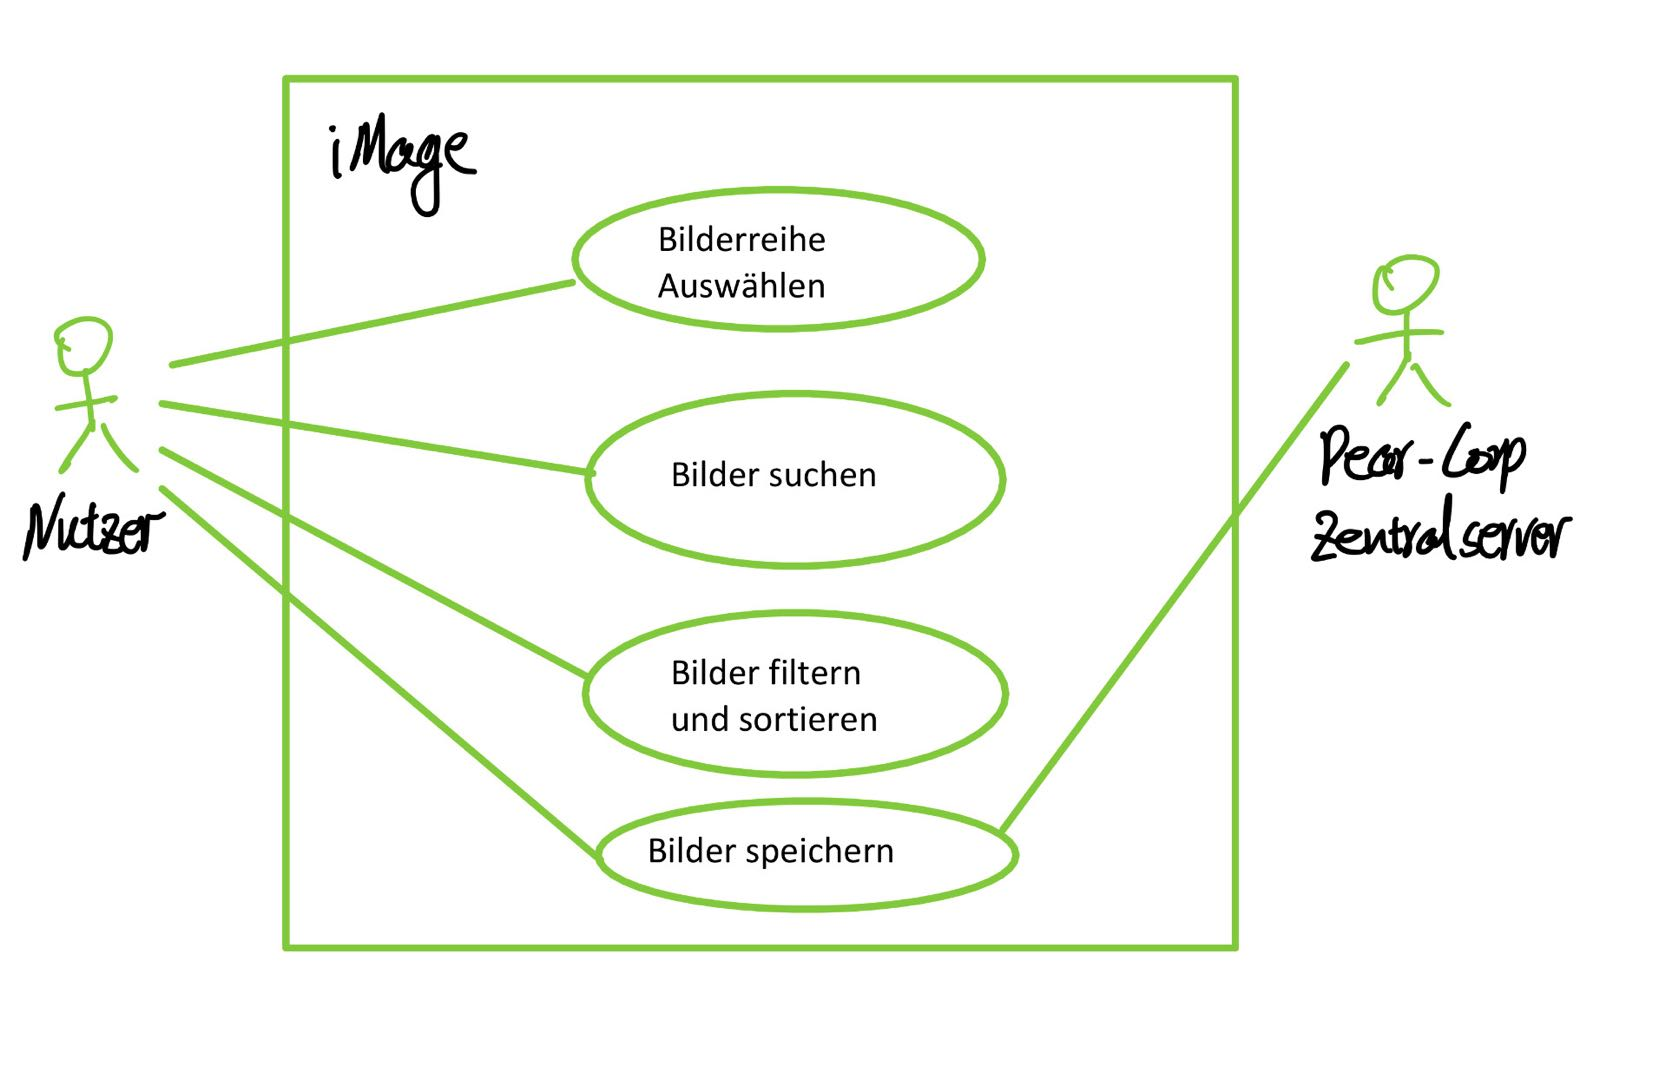
\includegraphics[width=0.8\textwidth]{Anwendungsfall.jpg}
\end{center}

\section{Durchführbarkeitsuntersuchung}

\subsection{Prüfen der fachlichen Durchführbarkeit}
\begin{itemize}
	\item Technische Infrastruktur vorhaden oder leicht beschaffbar.
\end{itemize}

\subsection{Prüfen alternativer Lösungsvorschläge}
\begin{itemize}
	\item Verwendung vorhandener Bilderverarbeitungsalgorithmen möglich.
\end{itemize}
\subsection{Prüfen der personellen Durchführbarkeit}
\begin{itemize}
	\item Fachkräfte in andere Projekte eingebunden
\end{itemize}
\subsection{Prüfen der Risiken}
\begin{itemize}
	\item Kunden stark interessiert an dieser Funktion.
\end{itemize}
\subsection{Prüfen der ökonomischen Durchführbarkeit}
\begin{itemize}
	\item Aufwands- und Terminschätzung: Aufwand machbar bis zur Veröffentlichung
\end{itemize}
\subsection{Rechtliche Gesichtspunkte}
\begin{itemize}
	\item Patente der Firma Abode prüfen und ggf. ankaufen
\end{itemize}
\end{document}
